\documentclass[12pt, letterpaper, twoside]{report}
\usepackage[utf8]{inputenc}
\usepackage{graphicx}
\usepackage{verbatim}
\graphicspath{{images/}}
\usepackage{url}

\title{\textbf{autorank}}
\author{Mohammad Sorkhian}
\date{2020 July 31}

\begin{document}

\maketitle

\chapter{Introduction}
\section{What is \textbf{autorank}}
Autorank is a simple Python package with one task: simplify the comparison between (multiple) paired populations. The performance measures on each data set are then the paired samples, the difference in the central tendency (e.g., the mean or median) can be used to rank the different algorithms.

The distribution of the populations must be analyzed with the Shapiro-Wilk test for normality and, depending on the normality with Levene's test or Bartlett's tests for homogeneity of the data. All this is already quite complex. This does not yet account for the adjustment of the significance level in case of repeated tests to achieve the desired family-wise significance. \\Additionally, not only the tests should be conducted, but good reporting of the results also include confidence intervals, effect sizes, and the decision of whether it is appropriate to report the mean value and standard deviation, or whether the median value and the median absolute deviation is more appropriate.

The goal of Autorank is to simplify the statistical analysis for non-experts. Autorank takes care of all of the above with a single function call. Additional functions allow the generation of appropriate plots, result tables, and even of a complete latex document. All that is required is the data about the populations is in a Pandas dataframe

\section{Practical implementation of \textbf{autorank}}
We have benefited this library to compare different countries worldwide in terms of their new \textit{Covid-19} detected cases and will present ten countries with highest volume in last month.

\chapter{Graphs}
\section{autorank Graph}
In this section we see the autorank plot
\begin{figure}[ht]
    \centering
    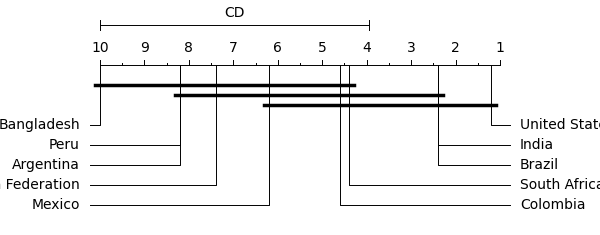
\includegraphics[width=0.8\textwidth]{autorank.png}
    \caption{autorank plot}
    \label{fig:autorank}
\end{figure} 

\section{matplotlib Garaph}
 In this section we see the top countries plot
\begin{figure}[ht]
    \centering
    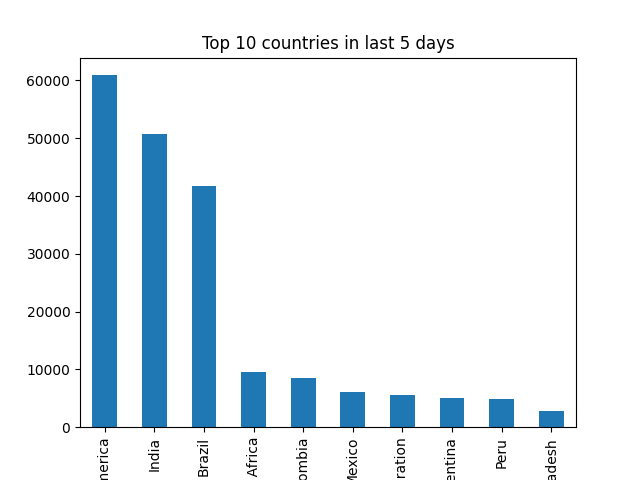
\includegraphics[width=0.8\textwidth]{TopCountries.png}
    \caption{Countries with highest rate of new \textit{Covid-19} detected cases}
    \label{fig:TopCountries}
\end{figure}

\chapter{autorank Reports}
 \verbatiminput{autorankReport.txt}
 \begin{abstract}
  autorank is a simple Python package with one task: simplify the comparison between (multiple) paired populations. This is, for example, required if the performance different machine learning algorithms or simulations should be compared on multiple data sets. The performance measures on each data set are then the paired samples, the difference in the central tendency (e.g., the mean or median) can be used to rank the different algorithms. In \ref{fig:autorank} you can see one output sample of this library
 \end{abstract}
 
@article{Herbold2020,
  doi = {10.21105/joss.02173},
  url = {\url{https://doi.org/10.21105/joss.02173}},
  year = {2020},
  publisher = {The Open Journal},
  volume = {5},
  number = {48},
  pages = {2173},
  author = {Steffen Herbold},
  title = {Autorank: A Python package for 
  automated ranking of classifiers},
  journal = {Journal of Open Source Software}
}

 \end{document}